\chapter{Background} \label{ch:background}

In this chapter, technical background of concepts needed to understand the work in this thesis is covered. Identity management concepts such as digital identity, identity access management, access control and access control models are explained.

\section{Blockchain} \label{ch:background-blockchain}

%\begin{description}
	\textbf{Blockchain}	refers to the technology that was used by Satoshi Nakamoto in \cite{nakamoto_bitcoin:_nodate} as the underlying building block of Bitcoin. It is based on the proposed solution to the problem of time-stamping data as described in \cite{haber_how_1991}, which uses hashes of data and links them in a chain, later on referred to as a chain of blocks (or block chain)  data structure introduced in 1991. Satoshi's paper and Bitcoin's implementation created an ever-growing ecosystem with multiple projects initially forked from Bitcoin as alternative cryptocurrencies (or alt-coins). A lot of enthusiasts envisioned general-purpose blockchain platforms which could potentially be used in a variety of use cases other than cryptocurrencies, such as, tokenization of assets, e-voting, supply chain, notarization, intellectual property protection, peer-to-peer financial transactions or settlements, and digital evidence \cite{noauthor_20_nodate}. To enable the creation of diverse applications, several blockchain platforms have been developed, as either public platforms targeting end-users or private aiming to support the enterprise sector \cite{noauthor_top_nodate}.    
%\end{description}

\begin{figure}[!h]
	\centering
	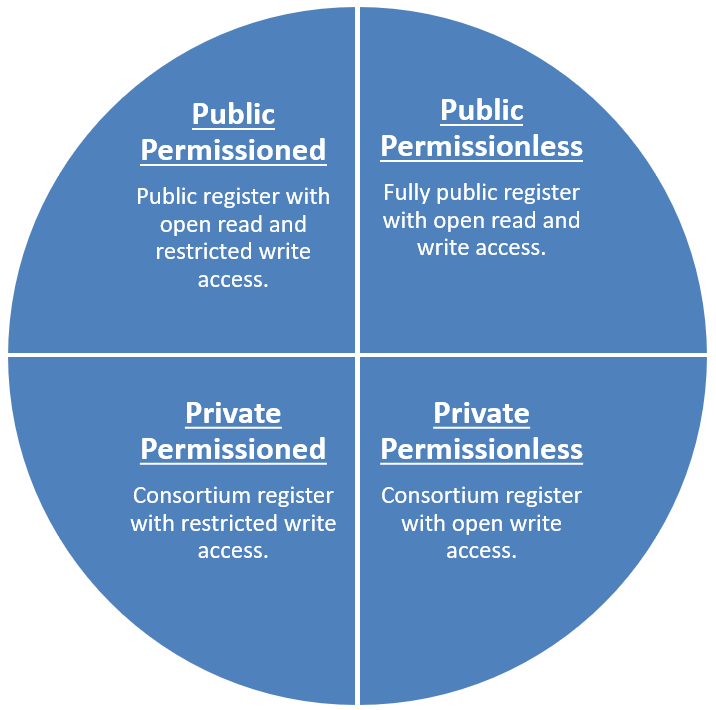
\includegraphics[width=80mm]{figs/ch2/bc-chart}
	\caption{Blockchain deployment types, based on \cite{rodrigues_technology-driven_nodate}}
	\label{fig:bc-deployment-types}
\end{figure}


The terms public and private in relation to blockhain platforms refer to the ability of an entity to be able to participate freely in the network. Participation to a blockchain platform might refer to any of several activities, such as, accessing the blockchain network freely, running an independent node or keeping a copy of the distributed ledger, participating in the consensus mechanism and executing functionality. 

A public blockchain is defined as a platform where anyone can participate and perform the activities stated above with no access control. Analogously, a private blockchain is defined as a platform where entities can only participate if they are granted access by the platform owner. The terms permissioned and permissionless, in relation to Swiss Educhain and the scope of this thesis, refer to the permission to write in the distributed ledger. Figure \ref{fig:bc-deployment-types} presents a high-level separation of the different blockchain platform types with respect to access control.

For the Swiss Educhain service, a hybrid approach has been chosen to combine a public permissionless blockchain with a private permissioned blockchain. The need for a private permissioned blockchain platform derives from the architectural requirements analysis in Section \ref{ssec:architectural-requirements}. For the scope of this thesis and the identity management of Swiss Educhain participants only the private permissioned blockchain is relevant. 


\section{Identity} \label{sec:background-identity}

Identity and access management (IAM) is a vast topic that consists of a plethora of processes, frameworks and technical implementation solutions. In this section, the foundational theoretical background of identity is explained with an emphasis only on the aspects that are relevant to this work. In Section \ref{sec:background-iam} Identity and Access Management is explained in more detail.

\subsection{Digital Identity}

The notion of identity is a subject that precedes the digital era and can be defined as something different depending on the unique perspective from which it is examined \cite{sociology-identity}, \cite{psychology-identity}. When identity is mentioned in this work it refers to the digital identity as seen from the prism of information technology and computer science.

An informal way to describe what is an identity would be the set of unique characteristics or attributes of an entity (human or not) which can uniquely identity this entity and differentiate it from other ones. As stated in \cite{digital-identity-guidelines} by Grassi et al., "a single definition is widely debated internationally", therefore the following definition aims to explain the concept rather than provide a formal definition. According to \cite{digital-identity-techopedia} a \textbf{digital identity} is defined as: 

\begin{description}
	\itemsep0em
	\item[] "\dots an online or networked identity adopted or claimed in cyberspace by an individual, organization or electronic device. These users may also project more than one digital identity through multiple communities. A digital identity is linked to one or more digital identifiers, like an email address, URL or domain name."
\end{description}

As it is inherently very hard to prove ownership of a digital identity and associate it with a specific entity (human or technical), especially over the Internet or any network, various processes and techniques have been developed as a potential solution to prevent identity impersonation and other attacks \cite{digital-identity-guidelines}. A brief high-level overview of such processes and frameworks is presented in Section \ref{sec:background-iam}.

\subsection{Self-Sovereign Identity}

A traditional identity, digital or not, is usually verified by an identity provider (in digital systems) or by an authority such as a government or a trusted third party to uniquely map an identity to an entity and prevent impersonation. The official documents or the digital accounts are issued on behalf of the entity, which is the identity owner, and handed over to them after a verification procedure is completed. An unconventional and different paradigm has emerged historically known as \textbf{self-ownership} or \textbf{individual sovereignty} through various political philosophies such as liberalism and anarchism \cite{kohl_politics_1991}. Stemming from these, a more recent evolution of this notion is the \textbf{self-sovereign identity} (SSI). 

Christopher Allen in \cite{ssi-allen} identifies four distinct phases in the evolution of identity:

\begin{enumerate}
	\itemsep0em
	\item \textbf{Centralized Identity} administrative control by a single authority or hierarchy,
	\item \textbf{Federated Identity} administrative control by multiple, federated authorities,
	\item \textbf{User-Centric Identity} individual or administrative control across multiple authorities without requiring a federation,
	\item \textbf{Self-Sovereign Identity} individual control across any number of authorities.
\end{enumerate}

According to Allen \cite{ssi-allen} a formal definition what is self-sovereign identity cannot be proposed, but he enumerates a set of principles that are meant to "\dots provoke a discussion about what is truly important.":

\begin{enumerate}
	\itemsep0em %can even put negative values to reduce vertical space, alternative solution is here -> https://tex.stackexchange.com/questions/6081/reduce-space-between-enumerated-items
	\item \textbf{Existence} - users must have an independent existence.
	\item \textbf{Control} - users must control their identities.
	\item \textbf{Access} - users must have access to their own data.
	\item \textbf{Transparency} - systems and algorithms must be transparent. 
	\item \textbf{Persistence} - identities must be long-lived.
	\item \textbf{Portability} - information and services about identity must be transportable.
	\item \textbf{Interoperability} - identities should be as widely usable as possible.
	\item \textbf{Consent} - users must agree to the use of their identity.
	\item \textbf{Minimalization} - disclosure of claims must be minimized.
	\item \textbf{Protection} - the rights of users must be protected.
\end{enumerate}

Partial realizations of the self-sovereign identity vision have been technically possible utilizing, blockchain, decentralized systems, consensus algorithms and applied cryptography. Some popular self-sovereign identity platforms include Sovrin \cite{sovrin-website}, uPort \cite{uport-website} and ShoCard \cite{shocard-website}. A detailed explanation and analysis of the platforms is provided in \cite{ssi-comparison}.


\section{Identity and Access Management} \label{sec:background-iam}

The existence of digital identities and their usage in computing systems, created the need to effectively manage digital accounts, verify their owners, provide fine-grained access to resources and allow for account lifecycle management via create, read, update and delete (CRUD) operations. 

\textbf{Identity and access management (IAM)} is defined by Gartner \cite{iam-definition-gartner} as: \newline
 "\dots the discipline that enables the right individuals to access the right resources at the right times for the right reasons."

In order for any IAM system to provide access to users to different resources, distinct steps need to be executed as part of the overall \textbf{access control} process. These steps can be identified in a high-level as \emph{Identification}, \emph{Authentication} and \emph{Authorization}; a detailed explanation of the access control process is given in Section \ref{ssec:access-control}. There exist multiple ways to implement this functionality, resulting in different access control models, the more relevant ones to this thesis' work are explained in Section \ref{ssec:access-control-models}. How accounts or roles are created is not analyzed in this chapter since it is a subjective matter greatly affected by the system's design and requirements.

\subsection{Access Control} \label{ssec:access-control}

\textbf{Access control} in the computer security context, can be described as the process through which users are granted access and certain privileges to systems, resources or information based on a set of credentials, assumed role or identity characteristics \cite{access-control-definition-techopedia}, \cite{access-control-definition-csoonline}, \cite{access-control-definition-searchsecurity}. The access control process has three distinct steps:

\begin{description}
	\itemsep0em
	\item[Identification] \hfill \\
	In computing systems, identification can be informally described as the ability to uniquely identify a user's account and associate it with an entity, (e.g. with a unique username for digital systems or an access card for physical access), with several more formalized definitions listed in \cite{identification-def-nist}. 
	%Additionally, some applications require that a user's account is mapped through an one-to-one relationship to the identity of a real person, achieved via physical identity documents verification (KYC process) and uses a drivers license, a passport or a national id. 
	\item[Authentication] \hfill \\
	Authentication "\dots  refers to an electronic process that allows for the electronic identification of a natural or legal person. Additionally, authentication may also confirm the origin and integrity of data in electronic form, such as the issuance of a digital certificate to attest to the authenticity of a website." \cite{authentication-definition-cryptomathic}. 
	%https://en.wikipedia.org/wiki/Authentication#Authentication_factors
	In general, authentication can be performed against three \textbf{authentication factors}:
	\begin{description}
		\itemsep0em
		\item \textbf{Knowledge} this includes passwords or passphrases, a personal identification number (PIN) or a response to a pre-selected security question. 
		\item \textbf{Ownership} this includes something that a user possesses, e.g. an access card, an one-time password (OTP) token or a specific phone number.
		\item \textbf{Inherence} this could be something that a user is, e.g. biometric identifiers such as facial, fingerprint or retinal pattern recognition. \cite{authentication-definition-cryptomathic}
	\end{description}
	Using one or more of the aforementioned factors, there are four main \textbf{types of authentication}, described below in order based on the increasing levels of security as explained in \cite{authentication-definition-cryptomathic}:
	\begin{description}
		\itemsep0em
		\item \textbf{Single-factor} uses only one of the components, it is considered a method easily susceptible to impersonation or replay attacks and is not preferred in most modern systems.
		\item \textbf{Two-factor (2FA)} combines two factors, e.g. something a user has and something a user knows, is considered safer and is available to the majority of computing systems. 
		\item \textbf{Multi-factor (MFA)} is similar to 2FA but combines more than two authentication factors to achieve enhanced security.
		\item \textbf{Strong Authentication} was requested by the European Banking Authority (EBA) \cite{strong-authentication} to provide enhanced security for financial customers. It provides specific requirements such as, usage of \textbf{a minimum of two mutually independent factors} and at least one element that is \textbf{non-reusable} and \textbf{non-replicable}. A detailed opinion on the elements of strong authentication is provided in a report published by the EBA \cite{strong-authentication-opinion}.
	\end{description}
	\item[Authorization] \hfill \\
	Authorization "\dots refers to the process of granting privileges to processes and, ultimately, users." \cite{authentication-def-ietf}. Authorization always succeeds authentication, after a user's claim of account ownership has been confirmed, the user is granted access to a set of resources based on either account information, assumed roles, membership in a group or organization, or other authorization rules \cite{auth-rules-ibm}. 
\end{description}

\subsection{Access Control Models} \label{ssec:access-control-models}
%https://en.wikipedia.org/wiki/Access_control#Access_control_models

A variety of access control models exists to serve diverse purposes and implement unique custom access control management policies. Briefly defined are the models related to this work:

\begin{description}
	\itemsep0em
	\item \textbf{Attribute-based Access Control (ABAC)} is defined as "An access control method where subject requests to perform	operations on objects are granted or denied based on assigned attributes of the subject, assigned attributes of the object, environment conditions, and a set of policies that are specified in terms of those attributes and conditions." \cite{abac-nist}. %The attributes of a user's account are evaluated against a policy and simple or fine-grained access is provided to the resource requested. %access rights are granted to users through the use of policies which evaluate attributes (user attributes, resource attributes and environment conditions). CITATION -> % http://nvlpubs.nist.gov/nistpubs/specialpublications/NIST.sp.800-162.pdf.
	%\item\textbf{Organization-based Access Control (OrBAC)} description %https://web.archive.org/web/20170610205017/http://orbac.org/
	\item\textbf{Role-Based Access Control (RBAC)} is defined as "Access control based on user roles (i.e., a collection of access authorizations a user receives based on an explicit or implicit assumption of a given role). Role permissions may be inherited through a role hierarchy and typically reflect the permissions needed to perform defined functions within an organization. A given role may apply to a single individual or to several individuals." \cite{rbac-def-nist-glossary}, \cite{rbac-def-nist}.
	
	
	%https://en.wikipedia.org/wiki/Access_control#Access_control_models https://biztechmagazine.com/article/2019/08/access-control-models-how-navigate-changing-security-frontiers
	%\item\textbf{Rule-Based Access Control (RAC)} description %https://en.wikipedia.org/wiki/Access_control#Access_control_models https://biztechmagazine.com/article/2019/08/access-control-models-how-navigate-changing-security-frontiers
\end{description}